% Created 2019-01-10 Thu 11:11
% Intended LaTeX compiler: pdflatex
\documentclass[11pt]{article}
\usepackage[utf8]{inputenc}
\usepackage[T1]{fontenc}
\usepackage{graphicx}
\usepackage{grffile}
\usepackage{longtable}
\usepackage{wrapfig}
\usepackage{rotating}
\usepackage[normalem]{ulem}
\usepackage{amsmath}
\usepackage{textcomp}
\usepackage{amssymb}
\usepackage{capt-of}
\usepackage{hyperref}
\usepackage[margin=1in]{geometry}
\author{Till Poppels}
\date{\today}
\title{Code to reproduce statistics and graphs in Poppels \& Kehler (2018, Glossa)}
\hypersetup{
 pdfauthor={Till Poppels},
 pdftitle={Code to reproduce statistics and graphs in Poppels \& Kehler (2018, Glossa)},
 pdfkeywords={},
 pdfsubject={},
 pdfcreator={Emacs 25.1.1 (Org mode 9.2)}, 
 pdflang={English}}
\begin{document}

\maketitle
\tableofcontents

\begin{verbatim}

require("tidyverse")
require("forcats")
require("ggrepel")
require("lme4")
source("expt-01-pre-processing.R")
source("expt-02-pre-processing.R")
source("expt-03-pre-processing.R")
source("expt-04-pre-processing.R")
d1 <- read_rds("../data/expt-01-clean-data.rds")
d2 <- read_rds("../data/expt-02-clean-data.rds")
d3 <- read_rds("../data/expt-03-clean-data.rds")
d4 <- read_rds("../data/expt-04-clean-data.rds")

\end{verbatim}

\begin{verbatim}



|Experiment | Participants recruited| excluded| remaining|
|:----------|----------------------:|--------:|---------:|
|Expt 1     |                     30|        1|        29|
|Expt 2     |                     60|        0|        60|
|Expt 3     |                     30|        2|        28|
|Expt 4     |                     31|        5|        26|
\end{verbatim}



\begin{figure}[htbp]
\centering
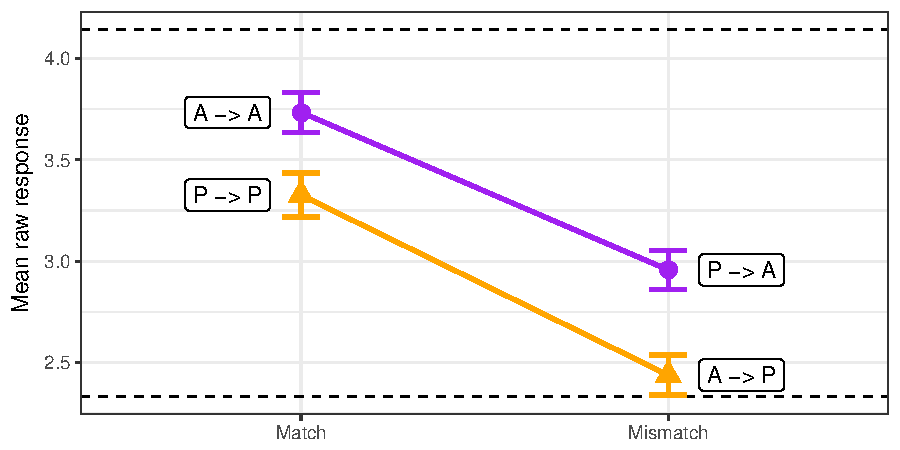
\includegraphics[width=.9\linewidth]{img/expt-01-graph.pdf}
\caption{Results from Expt 1.}
\end{figure}

\begin{verbatim}

Linear mixed model fit by maximum likelihood  ['lmerMod']
Formula: response ~ mismatch + voice.ellipsis + mismatch:voice.ellipsis +  
    (1 + mismatch * voice.ellipsis | sid) + (1 + mismatch * voice.ellipsis |  
    itemNo)
   Data: tmp

     AIC      BIC   logLik deviance df.resid 
  1679.0   1787.0   -814.5   1629.0      531 

Scaled residuals: 
     Min       1Q   Median       3Q      Max 
-2.95231 -0.56201  0.01544  0.62020  3.04203 

Random effects:
 Groups   Name                    Variance Std.Dev. Corr             
 sid      (Intercept)             0.259349 0.50926                   
          mismatch                0.079187 0.28140   0.25            
          voice.ellipsis          0.041940 0.20479  -0.43  0.48      
          mismatch:voice.ellipsis 0.013549 0.11640   0.69  0.56 -0.45
 itemNo   (Intercept)             0.076148 0.27595                   
          mismatch                0.029970 0.17312  -0.98            
          voice.ellipsis          0.020334 0.14260   0.70 -0.54      
          mismatch:voice.ellipsis 0.007858 0.08865  -0.90  0.97 -0.32
 Residual                         0.851430 0.92273                   
Number of obs: 556, groups:  sid, 29; itemNo, 24

Fixed effects:
                        Estimate Std. Error t value
(Intercept)              3.11560    0.11689  26.655
mismatch                -0.40806    0.07437  -5.487
voice.ellipsis          -0.23905    0.06196  -3.858
mismatch:voice.ellipsis -0.02933    0.04840  -0.606

Correlation of Fixed Effects:
            (Intr) msmtch vc.llp
mismatch    -0.083              
voice.llpss -0.055  0.086       
msmtch:vc.l  0.087  0.352 -0.184

Data: tmp
Models:
m.mismatch: response ~ 1 + voice.ellipsis + mismatch:voice.ellipsis + (1 + 
m.mismatch:     mismatch * voice.ellipsis | sid) + (1 + mismatch * voice.ellipsis | 
m.mismatch:     itemNo)
m: response ~ mismatch + voice.ellipsis + mismatch:voice.ellipsis + 
m:     (1 + mismatch * voice.ellipsis | sid) + (1 + mismatch * voice.ellipsis | 
m:     itemNo)
           Df    AIC    BIC  logLik deviance  Chisq Chi Df Pr(>Chisq)    
m.mismatch 24 1698.9 1802.6 -825.43   1650.9                             
m          25 1679.0 1787.0 -814.50   1629.0 21.863      1  2.928e-06 ***
---
codes:  0 ‘***’ 0.001 ‘**’ 0.01 ‘*’ 0.05 ‘.’ 0.1 ‘ ’ 1

Data: tmp
Models:
m.voice: response ~ mismatch + 1 + mismatch:voice.ellipsis + (1 + mismatch * 
m.voice:     voice.ellipsis | sid) + (1 + mismatch * voice.ellipsis | 
m.voice:     itemNo)
m: response ~ mismatch + voice.ellipsis + mismatch:voice.ellipsis + 
m:     (1 + mismatch * voice.ellipsis | sid) + (1 + mismatch * voice.ellipsis | 
m:     itemNo)
        Df  AIC    BIC  logLik deviance  Chisq Chi Df Pr(>Chisq)    
m.voice 24 1689 1792.6 -820.47     1641                             
m       25 1679 1787.0 -814.50     1629 11.947      1  0.0005473 ***
---
codes:  0 ‘***’ 0.001 ‘**’ 0.01 ‘*’ 0.05 ‘.’ 0.1 ‘ ’ 1

Data: tmp
Models:
m.interaction: response ~ mismatch + voice.ellipsis + 1 + (1 + mismatch * voice.ellipsis | 
m.interaction:     sid) + (1 + mismatch * voice.ellipsis | itemNo)
m: response ~ mismatch + voice.ellipsis + mismatch:voice.ellipsis + 
m:     (1 + mismatch * voice.ellipsis | sid) + (1 + mismatch * voice.ellipsis | 
m:     itemNo)
              Df    AIC    BIC  logLik deviance  Chisq Chi Df Pr(>Chisq)
m.interaction 24 1677.4 1781.1 -814.68   1629.4                         
m             25 1679.0 1787.0 -814.50   1629.0 0.3645      1      0.546
\end{verbatim}

\begin{figure}[htbp]
\centering
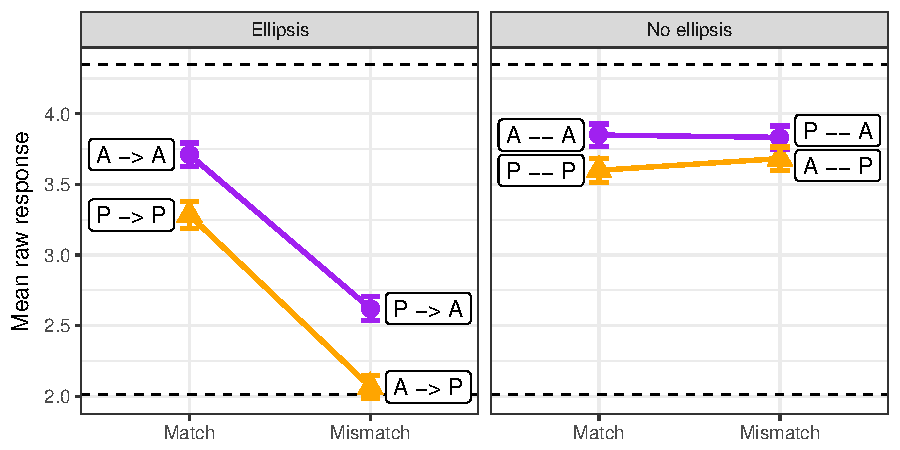
\includegraphics[width=.9\linewidth]{img/expt-02-graph.pdf}
\caption{Results from Expt 2.}
\end{figure}

\begin{verbatim}

Linear mixed model fit by maximum likelihood  ['lmerMod']
Formula: response ~ mismatch + voice.ellipsis + mismatch:voice.ellipsis +  
    (1 + mismatch * voice.ellipsis | sid) + (1 + mismatch * voice.ellipsis |  
    itemNo)
   Data: tmp

     AIC      BIC   logLik deviance df.resid 
  2078.3   2192.7  -1014.1   2028.3      695 

Scaled residuals: 
    Min      1Q  Median      3Q     Max 
-2.3648 -0.6002  0.0096  0.6058  3.2750 

Random effects:
 Groups   Name                    Variance Std.Dev. Corr             
 sid      (Intercept)             0.230502 0.48011                   
          mismatch                0.052075 0.22820   0.38            
          voice.ellipsis          0.008361 0.09144   0.68  0.07      
          mismatch:voice.ellipsis 0.022332 0.14944  -0.32  0.07 -0.91
 itemNo   (Intercept)             0.153439 0.39171                   
          mismatch                0.088899 0.29816  -0.82            
          voice.ellipsis          0.065489 0.25591   0.00 -0.44      
          mismatch:voice.ellipsis 0.013957 0.11814  -0.14  0.06  0.17
 Residual                         0.687476 0.82914                   
Number of obs: 720, groups:  sid, 60; itemNo, 24

Fixed effects:
                        Estimate Std. Error t value
(Intercept)              2.91866    0.10583  27.578
mismatch                -0.57437    0.07440  -7.720
voice.ellipsis          -0.24987    0.06187  -4.039
mismatch:voice.ellipsis -0.03182    0.04377  -0.727

Correlation of Fixed Effects:
            (Intr) msmtch vc.llp
mismatch    -0.419              
voice.llpss  0.077 -0.303       
msmtch:vc.l -0.144  0.041  0.001

Data: tmp
Models:
m.mismatch: response ~ 1 + voice.ellipsis + mismatch:voice.ellipsis + (1 + 
m.mismatch:     mismatch * voice.ellipsis | sid) + (1 + mismatch * voice.ellipsis | 
m.mismatch:     itemNo)
m: response ~ mismatch + voice.ellipsis + mismatch:voice.ellipsis + 
m:     (1 + mismatch * voice.ellipsis | sid) + (1 + mismatch * voice.ellipsis | 
m:     itemNo)
           Df    AIC    BIC  logLik deviance  Chisq Chi Df Pr(>Chisq)    
m.mismatch 24 2107.9 2217.8 -1030.0   2059.9                             
m          25 2078.3 2192.8 -1014.1   2028.3 31.646      1   1.85e-08 ***
---
codes:  0 ‘***’ 0.001 ‘**’ 0.01 ‘*’ 0.05 ‘.’ 0.1 ‘ ’ 1

Data: tmp
Models:
m.voice: response ~ mismatch + 1 + mismatch:voice.ellipsis + (1 + mismatch * 
m.voice:     voice.ellipsis | sid) + (1 + mismatch * voice.ellipsis | 
m.voice:     itemNo)
m: response ~ mismatch + voice.ellipsis + mismatch:voice.ellipsis + 
m:     (1 + mismatch * voice.ellipsis | sid) + (1 + mismatch * voice.ellipsis | 
m:     itemNo)
        Df    AIC    BIC  logLik deviance  Chisq Chi Df Pr(>Chisq)    
m.voice 24 2088.7 2198.6 -1020.4   2040.7                             
m       25 2078.3 2192.8 -1014.1   2028.3 12.459      1   0.000416 ***
---
codes:  0 ‘***’ 0.001 ‘**’ 0.01 ‘*’ 0.05 ‘.’ 0.1 ‘ ’ 1

Data: tmp
Models:
m.interaction: response ~ mismatch + voice.ellipsis + 1 + (1 + mismatch * voice.ellipsis | 
m.interaction:     sid) + (1 + mismatch * voice.ellipsis | itemNo)
m: response ~ mismatch + voice.ellipsis + mismatch:voice.ellipsis + 
m:     (1 + mismatch * voice.ellipsis | sid) + (1 + mismatch * voice.ellipsis | 
m:     itemNo)
              Df    AIC    BIC  logLik deviance  Chisq Chi Df Pr(>Chisq)
m.interaction 24 2076.8 2186.7 -1014.4   2028.8                         
m             25 2078.3 2192.8 -1014.1   2028.3 0.5236      1     0.4693
\end{verbatim}

\begin{verbatim}

Linear mixed model fit by maximum likelihood  ['lmerMod']
Formula: response ~ mismatch + voice.ellipsis + mismatch:voice.ellipsis +  
    (1 + mismatch * voice.ellipsis | sid) + (1 + mismatch * voice.ellipsis |  
    itemNo)
   Data: tmp

     AIC      BIC   logLik deviance df.resid 
  2055.1   2169.5  -1002.5   2005.1      695 

Scaled residuals: 
    Min      1Q  Median      3Q     Max 
-3.3345 -0.6042  0.0939  0.5989  2.3103 

Random effects:
 Groups   Name                    Variance  Std.Dev. Corr             
 sid      (Intercept)             0.1974582 0.44436                   
          mismatch                0.0081874 0.09048   0.10            
          voice.ellipsis          0.0006514 0.02552  -0.52 -0.91      
          mismatch:voice.ellipsis 0.0077367 0.08796  -0.39  0.87 -0.59
 itemNo   (Intercept)             0.2017072 0.44912                   
          mismatch                0.0111075 0.10539   0.30            
          voice.ellipsis          0.0422154 0.20546  -0.18 -0.59      
          mismatch:voice.ellipsis 0.0217571 0.14750   0.20  0.97 -0.39
 Residual                         0.7276855 0.85304                   
Number of obs: 720, groups:  sid, 60; itemNo, 24

Fixed effects:
                        Estimate Std. Error t value
(Intercept)              3.74366    0.11275  33.202
mismatch                 0.01723    0.04021   0.428
voice.ellipsis          -0.10011    0.05277  -1.897
mismatch:voice.ellipsis  0.03061    0.04531   0.676

Correlation of Fixed Effects:
            (Intr) msmtch vc.llp
mismatch     0.145              
voice.llpss -0.134 -0.269       
msmtch:vc.l  0.060  0.409 -0.216

Data: tmp
Models:
m.mismatch: response ~ 1 + voice.ellipsis + mismatch:voice.ellipsis + (1 + 
m.mismatch:     mismatch * voice.ellipsis | sid) + (1 + mismatch * voice.ellipsis | 
m.mismatch:     itemNo)
m: response ~ mismatch + voice.ellipsis + mismatch:voice.ellipsis + 
m:     (1 + mismatch * voice.ellipsis | sid) + (1 + mismatch * voice.ellipsis | 
m:     itemNo)
           Df    AIC    BIC  logLik deviance  Chisq Chi Df Pr(>Chisq)
m.mismatch 24 2053.2 2163.2 -1002.6   2005.2                         
m          25 2055.1 2169.6 -1002.5   2005.1 0.1831      1     0.6688

Data: tmp
Models:
m.voice: response ~ mismatch + 1 + mismatch:voice.ellipsis + (1 + mismatch * 
m.voice:     voice.ellipsis | sid) + (1 + mismatch * voice.ellipsis | 
m.voice:     itemNo)
m: response ~ mismatch + voice.ellipsis + mismatch:voice.ellipsis + 
m:     (1 + mismatch * voice.ellipsis | sid) + (1 + mismatch * voice.ellipsis | 
m:     itemNo)
        Df    AIC    BIC  logLik deviance  Chisq Chi Df Pr(>Chisq)  
m.voice 24 2056.4 2166.3 -1004.2   2008.4                           
m       25 2055.1 2169.6 -1002.5   2005.1 3.3338      1    0.06787 .
---
codes:  0 ‘***’ 0.001 ‘**’ 0.01 ‘*’ 0.05 ‘.’ 0.1 ‘ ’ 1

Data: tmp
Models:
m.interaction: response ~ mismatch + voice.ellipsis + 1 + (1 + mismatch * voice.ellipsis | 
m.interaction:     sid) + (1 + mismatch * voice.ellipsis | itemNo)
m: response ~ mismatch + voice.ellipsis + mismatch:voice.ellipsis + 
m:     (1 + mismatch * voice.ellipsis | sid) + (1 + mismatch * voice.ellipsis | 
m:     itemNo)
              Df    AIC    BIC  logLik deviance  Chisq Chi Df Pr(>Chisq)
m.interaction 24 2053.5 2163.4 -1002.8   2005.5                         
m             25 2055.1 2169.6 -1002.5   2005.1 0.4532      1     0.5008
\end{verbatim}


\begin{figure}[htbp]
\centering
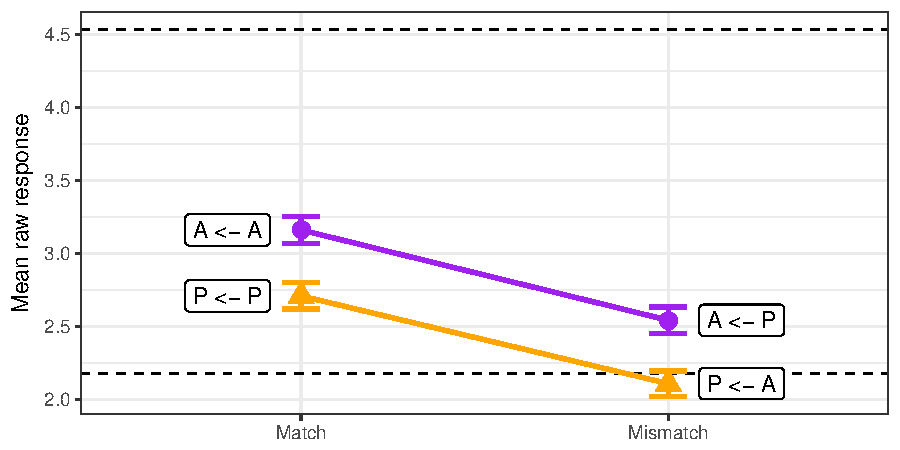
\includegraphics[width=.9\linewidth]{img/expt-03-graph.pdf}
\caption{Results from Expt 3.}
\end{figure}

\begin{verbatim}

Linear mixed model fit by maximum likelihood  ['lmerMod']
Formula: response ~ mismatch + voice.ellipsis + mismatch:voice.ellipsis +  
    (1 + mismatch * voice.ellipsis | sid) + (1 + mismatch * voice.ellipsis |  
    itemNo)
   Data: tmp

     AIC      BIC   logLik deviance df.resid 
  1943.6   2056.3   -946.8   1893.6      647 

Scaled residuals: 
     Min       1Q   Median       3Q      Max 
-3.13753 -0.63007 -0.06087  0.58549  2.72387 

Random effects:
 Groups   Name                    Variance Std.Dev. Corr             
 sid      (Intercept)             0.413559 0.64309                   
          mismatch                0.010954 0.10466   0.21            
          voice.ellipsis          0.009322 0.09655   0.29  0.42      
          mismatch:voice.ellipsis 0.012091 0.10996  -0.11 -0.16  0.58
 itemNo   (Intercept)             0.081690 0.28581                   
          mismatch                0.024887 0.15776  -0.69            
          voice.ellipsis          0.024614 0.15689  -0.41  0.11      
          mismatch:voice.ellipsis 0.005777 0.07600   0.25  0.49 -0.59
 Residual                         0.780822 0.88364                   
Number of obs: 672, groups:  sid, 28; itemNo, 24

Fixed effects:
                         Estimate Std. Error t value
(Intercept)              2.632243   0.139100  18.923
mismatch                -0.302273   0.051093  -5.916
voice.ellipsis          -0.229022   0.050325  -4.551
mismatch:voice.ellipsis  0.006914   0.043065   0.161

Correlation of Fixed Effects:
            (Intr) msmtch vc.llp
mismatch    -0.111              
voice.llpss -0.016  0.102       
msmtch:vc.l -0.007  0.080 -0.036

Data: tmp
Models:
m.mismatch: response ~ 1 + voice.ellipsis + mismatch:voice.ellipsis + (1 + 
m.mismatch:     mismatch * voice.ellipsis | sid) + (1 + mismatch * voice.ellipsis | 
m.mismatch:     itemNo)
m: response ~ mismatch + voice.ellipsis + mismatch:voice.ellipsis + 
m:     (1 + mismatch * voice.ellipsis | sid) + (1 + mismatch * voice.ellipsis | 
m:     itemNo)
           Df    AIC    BIC  logLik deviance  Chisq Chi Df Pr(>Chisq)    
m.mismatch 24 1964.1 2072.3 -958.04   1916.1                             
m          25 1943.6 2056.3 -946.78   1893.6 22.527      1  2.073e-06 ***
---
codes:  0 ‘***’ 0.001 ‘**’ 0.01 ‘*’ 0.05 ‘.’ 0.1 ‘ ’ 1

Data: tmp
Models:
m.voice: response ~ mismatch + 1 + mismatch:voice.ellipsis + (1 + mismatch * 
m.voice:     voice.ellipsis | sid) + (1 + mismatch * voice.ellipsis | 
m.voice:     itemNo)
m: response ~ mismatch + voice.ellipsis + mismatch:voice.ellipsis + 
m:     (1 + mismatch * voice.ellipsis | sid) + (1 + mismatch * voice.ellipsis | 
m:     itemNo)
        Df    AIC    BIC  logLik deviance  Chisq Chi Df Pr(>Chisq)    
m.voice 24 1956.4 2064.7 -954.22   1908.4                             
m       25 1943.6 2056.3 -946.78   1893.6 14.876      1  0.0001148 ***
---
codes:  0 ‘***’ 0.001 ‘**’ 0.01 ‘*’ 0.05 ‘.’ 0.1 ‘ ’ 1

Data: tmp
Models:
m.interaction: response ~ mismatch + voice.ellipsis + 1 + (1 + mismatch * voice.ellipsis | 
m.interaction:     sid) + (1 + mismatch * voice.ellipsis | itemNo)
m: response ~ mismatch + voice.ellipsis + mismatch:voice.ellipsis + 
m:     (1 + mismatch * voice.ellipsis | sid) + (1 + mismatch * voice.ellipsis | 
m:     itemNo)
              Df    AIC    BIC  logLik deviance  Chisq Chi Df Pr(>Chisq)
m.interaction 24 1941.6 2049.8 -946.79   1893.6                         
m             25 1943.6 2056.3 -946.78   1893.6 0.0257      1     0.8727
\end{verbatim}

\begin{figure}[htbp]
\centering
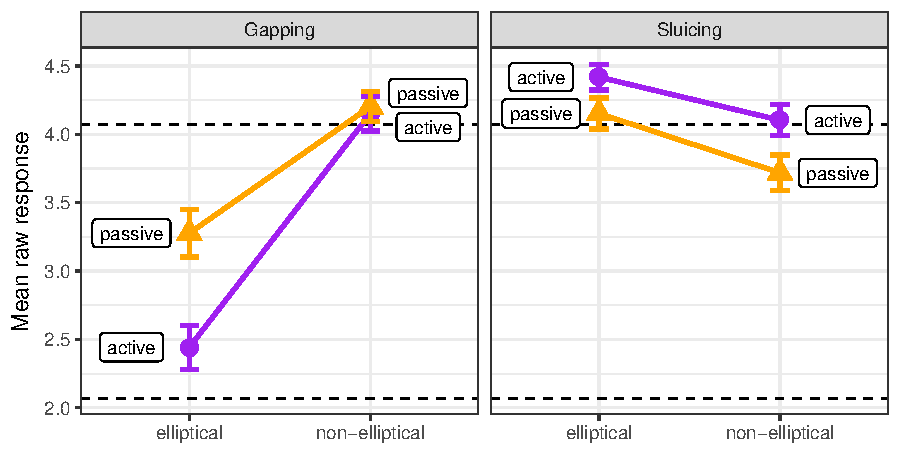
\includegraphics[width=.9\linewidth]{img/expt-04-graph.pdf}
\caption{Results from Expt 4 (pilot on gapping/sluicing).}
\end{figure}

\begin{verbatim}

Linear mixed model fit by maximum likelihood  ['lmerMod']
Formula: response ~ ellipsis + voice + ellipsis:voice + (1 + ellipsis |  
    sid) + (1 + ellipsis | itemNo)
   Data: tmp

     AIC      BIC   logLik deviance df.resid 
   865.4    905.8   -421.7    843.4      281 

Scaled residuals: 
    Min      1Q  Median      3Q     Max 
-3.7657 -0.5276  0.1071  0.5037  3.6453 

Random effects:
 Groups   Name        Variance Std.Dev. Corr
 sid      (Intercept) 0.46613  0.6827       
          ellipsis    0.19907  0.4462   0.47
 itemNo   (Intercept) 0.05694  0.2386       
          ellipsis    0.01967  0.1403   1.00
 Residual             0.75372  0.8682       
Number of obs: 292, groups:  sid, 26; itemNo, 12

Fixed effects:
               Estimate Std. Error t value
(Intercept)      3.5161     0.1602  21.943
ellipsis        -0.6515     0.1105  -5.893
voice            0.2029     0.1446   1.403
ellipsis:voice   0.1945     0.1025   1.898

Correlation of Fixed Effects:
            (Intr) ellpss voice
ellipsis    0.479              
voice       0.071  0.037       
ellipsis:vc 0.036  0.075  0.381

Data: tmp
Models:
m.ellipsis: response ~ 1 + voice + ellipsis:voice + (1 + ellipsis | sid) + 
m.ellipsis:     (1 + ellipsis | itemNo)
m: response ~ ellipsis + voice + ellipsis:voice + (1 + ellipsis | 
m:     sid) + (1 + ellipsis | itemNo)
           Df    AIC    BIC  logLik deviance  Chisq Chi Df Pr(>Chisq)    
m.ellipsis 10 885.59 922.36 -432.79   865.59                             
m          11 865.38 905.82 -421.69   843.38 22.209      1  2.446e-06 ***
---
codes:  0 ‘***’ 0.001 ‘**’ 0.01 ‘*’ 0.05 ‘.’ 0.1 ‘ ’ 1
\end{verbatim}

\begin{verbatim}

Linear mixed model fit by maximum likelihood  ['lmerMod']
Formula: response ~ ellipsis + voice + ellipsis:voice + (1 | sid) + (1 |  
    itemNo)
   Data: tmp

     AIC      BIC   logLik deviance df.resid 
   895.1    920.9   -440.6    881.1      285 

Scaled residuals: 
    Min      1Q  Median      3Q     Max 
-3.2743 -0.6396  0.0240  0.6495  2.9683 

Random effects:
 Groups   Name        Variance Std.Dev.
 sid      (Intercept) 0.46710  0.6835  
 itemNo   (Intercept) 0.06801  0.2608  
 Residual             0.97944  0.9897  
Number of obs: 292, groups:  sid, 26; itemNo, 12

Fixed effects:
               Estimate Std. Error t value
(Intercept)     3.51405    0.16552  21.230
ellipsis       -0.68132    0.05868 -11.610
voice           0.19603    0.14739   1.330
ellipsis:voice  0.19847    0.05833   3.403

Correlation of Fixed Effects:
            (Intr) ellpss voice
ellipsis    0.007              
voice       0.068  0.012       
ellipsis:vc 0.012  0.079  0.009

Data: tmp
Models:
m.voice: response ~ ellipsis + 1 + ellipsis:voice + (1 | sid) + (1 | itemNo)
m: response ~ ellipsis + voice + ellipsis:voice + (1 | sid) + (1 | 
m:     itemNo)
        Df    AIC    BIC  logLik deviance  Chisq Chi Df Pr(>Chisq)
m.voice  6 894.84 916.90 -441.42   882.84                         
m        7 895.14 920.88 -440.57   881.14 1.6971      1     0.1927
\end{verbatim}

\begin{verbatim}

Linear mixed model fit by maximum likelihood  ['lmerMod']
Formula: response ~ ellipsis + voice + ellipsis:voice + (1 + ellipsis:voice |  
    sid) + (1 + ellipsis:voice | itemNo)
   Data: tmp

     AIC      BIC   logLik deviance df.resid 
   873.1    913.6   -425.6    851.1      281 

Scaled residuals: 
    Min      1Q  Median      3Q     Max 
-3.6788 -0.5154  0.0076  0.5025  3.4711 

Random effects:
 Groups   Name           Variance  Std.Dev. Corr 
 sid      (Intercept)    0.4722091 0.68717       
          ellipsis:voice 0.2047110 0.45245  0.17 
 itemNo   (Intercept)    0.0589566 0.24281       
          ellipsis:voice 0.0008724 0.02954  -1.00
 Residual                0.7693439 0.87712       
Number of obs: 292, groups:  sid, 26; itemNo, 12

Fixed effects:
               Estimate Std. Error t value
(Intercept)      3.5192     0.1617  21.769
ellipsis        -0.6441     0.1043  -6.176
voice            0.2078     0.1457   1.427
ellipsis:voice   0.1955     0.1043   1.875

Correlation of Fixed Effects:
            (Intr) ellpss voice
ellipsis    0.015              
voice       0.070  0.149       
ellipsis:vc 0.100  0.078  0.017

Data: tmp
Models:
m.interaction: response ~ ellipsis + voice + 1 + (1 + ellipsis:voice | sid) + 
m.interaction:     (1 + ellipsis:voice | itemNo)
m: response ~ ellipsis + voice + ellipsis:voice + (1 + ellipsis:voice | 
m:     sid) + (1 + ellipsis:voice | itemNo)
              Df    AIC    BIC  logLik deviance  Chisq Chi Df Pr(>Chisq)  
m.interaction 10 874.38 911.15 -427.19   854.38                           
m             11 873.11 913.55 -425.55   851.11 3.2733      1    0.07042 .
---
codes:  0 ‘***’ 0.001 ‘**’ 0.01 ‘*’ 0.05 ‘.’ 0.1 ‘ ’ 1
\end{verbatim}

\begin{verbatim}

Linear mixed model fit by maximum likelihood  ['lmerMod']
Formula: response ~ ellipsis + voice + ellipsis:voice + (1 + ellipsis |  
    sid) + (1 + ellipsis | itemNo)
   Data: tmp

     AIC      BIC   logLik deviance df.resid 
   771.0    811.4   -374.5    749.0      281 

Scaled residuals: 
    Min      1Q  Median      3Q     Max 
-4.5137 -0.3243  0.1175  0.5674  2.6977 

Random effects:
 Groups   Name        Variance Std.Dev. Corr 
 sid      (Intercept) 0.278385 0.52762       
          ellipsis    0.006674 0.08169  -1.00
 itemNo   (Intercept) 0.031676 0.17798       
          ellipsis    0.004898 0.06999  -1.00
 Residual             0.628695 0.79290       
Number of obs: 292, groups:  sid, 26; itemNo, 12

Fixed effects:
               Estimate Std. Error t value
(Intercept)     4.08698    0.12598  32.441
ellipsis        0.18637    0.05341   3.489
voice          -0.15851    0.11508  -1.377
ellipsis:voice  0.03392    0.04978   0.681

Correlation of Fixed Effects:
            (Intr) ellpss voice 
ellipsis    -0.411              
voice       -0.055  0.008       
ellipsis:vc  0.008 -0.059 -0.305

Data: tmp
Models:
m.ellipsis: response ~ 1 + voice + ellipsis:voice + (1 + ellipsis | sid) + 
m.ellipsis:     (1 + ellipsis | itemNo)
m: response ~ ellipsis + voice + ellipsis:voice + (1 + ellipsis | 
m:     sid) + (1 + ellipsis | itemNo)
           Df    AIC    BIC  logLik deviance  Chisq Chi Df Pr(>Chisq)   
m.ellipsis 10 778.17 814.94 -379.09   758.17                            
m          11 770.98 811.43 -374.49   748.98 9.1862      1   0.002438 **
---
codes:  0 ‘***’ 0.001 ‘**’ 0.01 ‘*’ 0.05 ‘.’ 0.1 ‘ ’ 1
\end{verbatim}

\begin{verbatim}

Linear mixed model fit by maximum likelihood  ['lmerMod']
Formula: response ~ ellipsis + voice + ellipsis:voice + (1 | sid) + (1 |  
    itemNo)
   Data: tmp

     AIC      BIC   logLik deviance df.resid 
   895.1    920.9   -440.6    881.1      285 

Scaled residuals: 
    Min      1Q  Median      3Q     Max 
-3.2743 -0.6396  0.0240  0.6495  2.9683 

Random effects:
 Groups   Name        Variance Std.Dev.
 sid      (Intercept) 0.46710  0.6835  
 itemNo   (Intercept) 0.06801  0.2608  
 Residual             0.97944  0.9897  
Number of obs: 292, groups:  sid, 26; itemNo, 12

Fixed effects:
               Estimate Std. Error t value
(Intercept)     3.51405    0.16552  21.230
ellipsis       -0.68132    0.05868 -11.610
voice           0.19603    0.14739   1.330
ellipsis:voice  0.19847    0.05833   3.403

Correlation of Fixed Effects:
            (Intr) ellpss voice
ellipsis    0.007              
voice       0.068  0.012       
ellipsis:vc 0.012  0.079  0.009

Data: tmp
Models:
m.voice: response ~ ellipsis + 1 + ellipsis:voice + (1 | sid) + (1 | itemNo)
m: response ~ ellipsis + voice + ellipsis:voice + (1 | sid) + (1 | 
m:     itemNo)
        Df    AIC    BIC  logLik deviance  Chisq Chi Df Pr(>Chisq)
m.voice  6 894.84 916.90 -441.42   882.84                         
m        7 895.14 920.88 -440.57   881.14 1.6971      1     0.1927
\end{verbatim}

\begin{verbatim}

Linear mixed model fit by maximum likelihood  ['lmerMod']
Formula: response ~ ellipsis + voice + ellipsis:voice + (1 + ellipsis:voice |  
    sid) + (1 + ellipsis:voice | itemNo)
   Data: tmp

     AIC      BIC   logLik deviance df.resid 
   773.2    813.7   -375.6    751.2      281 

Scaled residuals: 
    Min      1Q  Median      3Q     Max 
-4.1556 -0.2981  0.1198  0.5876  2.4703 

Random effects:
 Groups   Name           Variance Std.Dev. Corr 
 sid      (Intercept)    0.278983 0.52819       
          ellipsis:voice 0.001288 0.03589  1.00 
 itemNo   (Intercept)    0.034419 0.18552       
          ellipsis:voice 0.003862 0.06214  -1.00
 Residual                0.633500 0.79593       
Number of obs: 292, groups:  sid, 26; itemNo, 12

Fixed effects:
               Estimate Std. Error t value
(Intercept)     4.08276    0.12692  32.169
ellipsis        0.18572    0.04731   3.926
voice          -0.15559    0.11505  -1.352
ellipsis:voice  0.03521    0.05089   0.692

Correlation of Fixed Effects:
            (Intr) ellpss voice 
ellipsis    -0.010              
voice       -0.057  0.130       
ellipsis:vc -0.041 -0.065 -0.011

Data: tmp
Models:
m.interaction: response ~ ellipsis + voice + 1 + (1 + ellipsis:voice | sid) + 
m.interaction:     (1 + ellipsis:voice | itemNo)
m: response ~ ellipsis + voice + ellipsis:voice + (1 + ellipsis:voice | 
m:     sid) + (1 + ellipsis:voice | itemNo)
              Df    AIC    BIC  logLik deviance  Chisq Chi Df Pr(>Chisq)
m.interaction 10 771.69 808.45 -375.84   751.69                         
m             11 773.21 813.66 -375.61   751.21 0.4751      1     0.4907
\end{verbatim}


\begin{verbatim}

R version 3.4.4 (2018-03-15)
Platform: x86_64-pc-linux-gnu (64-bit)
Running under: Ubuntu 16.04 LTS

Matrix products: default
BLAS: /usr/lib/libblas/libblas.so.3.6.0
LAPACK: /usr/lib/lapack/liblapack.so.3.6.0

locale:
 [1] LC_CTYPE=en_US.UTF-8       LC_NUMERIC=C              
 [3] LC_TIME=en_US.UTF-8        LC_COLLATE=en_US.UTF-8    
 [5] LC_MONETARY=en_US.UTF-8    LC_MESSAGES=en_US.UTF-8   
 [7] LC_PAPER=en_US.UTF-8       LC_NAME=C                 
 [9] LC_ADDRESS=C               LC_TELEPHONE=C            
[11] LC_MEASUREMENT=en_US.UTF-8 LC_IDENTIFICATION=C       

attached base packages:
[1] stats     graphics  grDevices utils     datasets  methods   base     

other attached packages:
 [1] bindrcpp_0.2.2  lme4_1.1-17     Matrix_1.2-3    ggrepel_0.7.0  
 [5] forcats_0.3.0   stringr_1.3.1   dplyr_0.7.4     purrr_0.2.4    
 [9] readr_1.1.1     tidyr_0.8.0     tibble_1.4.2    ggplot2_2.2.1  
[13] tidyverse_1.2.1

loaded via a namespace (and not attached):
 [1] xfun_0.4         tidyselect_0.2.4 reshape2_1.4.2   splines_3.4.4   
 [5] haven_1.1.1      lattice_0.20-33  colorspace_1.3-2 rlang_0.2.0     
 [9] pillar_1.2.1     nloptr_1.0.4     foreign_0.8-66   glue_1.3.0      
[13] modelr_0.1.1     readxl_1.0.0     bindr_0.1.1      plyr_1.8.4      
[17] munsell_0.4.3    gtable_0.2.0     cellranger_1.1.0 rvest_0.3.2     
[21] psych_1.8.3.3    labeling_0.3     knitr_1.21       parallel_3.4.4  
[25] highr_0.6        broom_0.4.4      Rcpp_0.12.16     scales_0.4.1    
[29] jsonlite_1.6     mnormt_1.5-5     hms_0.4.2        stringi_1.2.4   
[33] grid_3.4.4       cli_1.0.0        tools_3.4.4      magrittr_1.5    
[37] lazyeval_0.2.0   crayon_1.3.4     pkgconfig_2.0.1  MASS_7.3-45     
[41] xml2_1.2.0       lubridate_1.7.3  assertthat_0.2.0 minqa_1.2.4     
[45] httr_1.3.1       rstudioapi_0.7   R6_2.2.2         nlme_3.1-124    
[49] compiler_3.4.4
\end{verbatim}
\end{document}